% slides.tex
\documentclass{beamer}
\usetheme{default}

\title{Detecting Snow Cover on GPS Antenna}
\subtitle{ASEN6090 Final Project}
\author{Kyle Wolma\\Logan Finch\\Praveen Vikram\\}
\institute[CU-ASEN]{
  Department of Aerospace Engineering Sciences\\
  Colorado University\\
  \texttt{kyle.wolma@colorado.edu\\logan.finch@colorado.edu\\praveen.vikram@colorado.edu}
}
\date[April 2012]{April 13, 2012}

\begin{document}

%--- the titlepage frame -------------------------%
\begin{frame}[plain]
  \titlepage
\end{frame}

%--- outline frame -------------------------%
\begin{frame}{Outline}

\begin{itemize}
  \item Goals
  \item Sites 
  \item Parameters
  \item Site Photos
  \item Preliminary Plots
\end{itemize}

\end{frame}

\begin{frame}{Goals}
\begin{itemize}
  \item Generate an index representative of snow cover over GPS antenna.
  \item Considerations for Reflections study:
  \begin{itemize}
    \item How much of an effect will Snow cover directly over the antenna have on received signal power from lower elevation angles.
%    \item Ice may form on the side of antenna, which may cause problems.
%    \item Detect signal loss from archived direct signal power for each SV at binned elevation.  
  \end{itemize}
\end{itemize}
\end{frame}

%--- sites frame -------------------------%
\begin{frame}{Sites}

Sites for Primary Study
\begin{itemize}
  \item P360
  \item P101
\end{itemize}

Both the above sites have a digital camera installed on site.
\end{frame}

%--- p360 frame -------------------------%
\begin{frame}{P360 Summary}
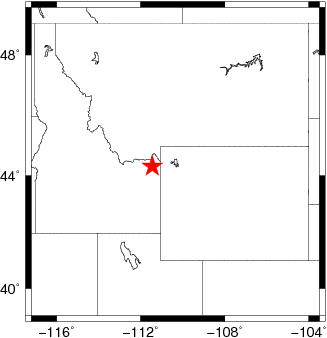
\includegraphics[width=0.4\linewidth]{img/map_p360.png}
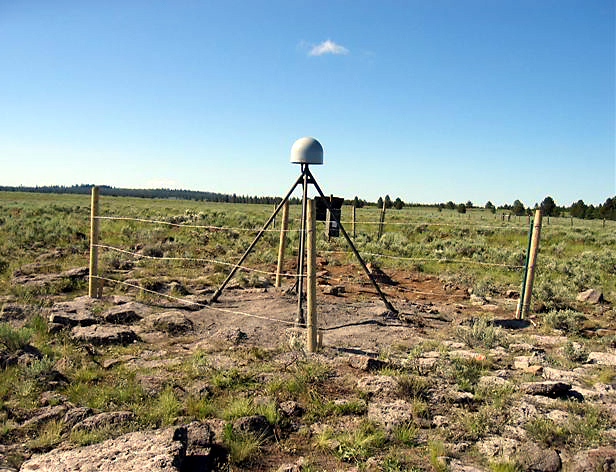
\includegraphics[width=0.5\linewidth]{img/overview.jpg}
\begin{itemize}  
  \item Station Installation Date: 2005-06-29 00:00:00
  \item Monument Installation Date: 2005-06-29 00:00:00
  \item Trimble NetRS Receiver
  \item TRM29659.00 Antenna with a Radome
\end{itemize}
\end{frame}

%--- p360 site photo frame -------------------------%
\begin{frame}{P360 - Feb 21}
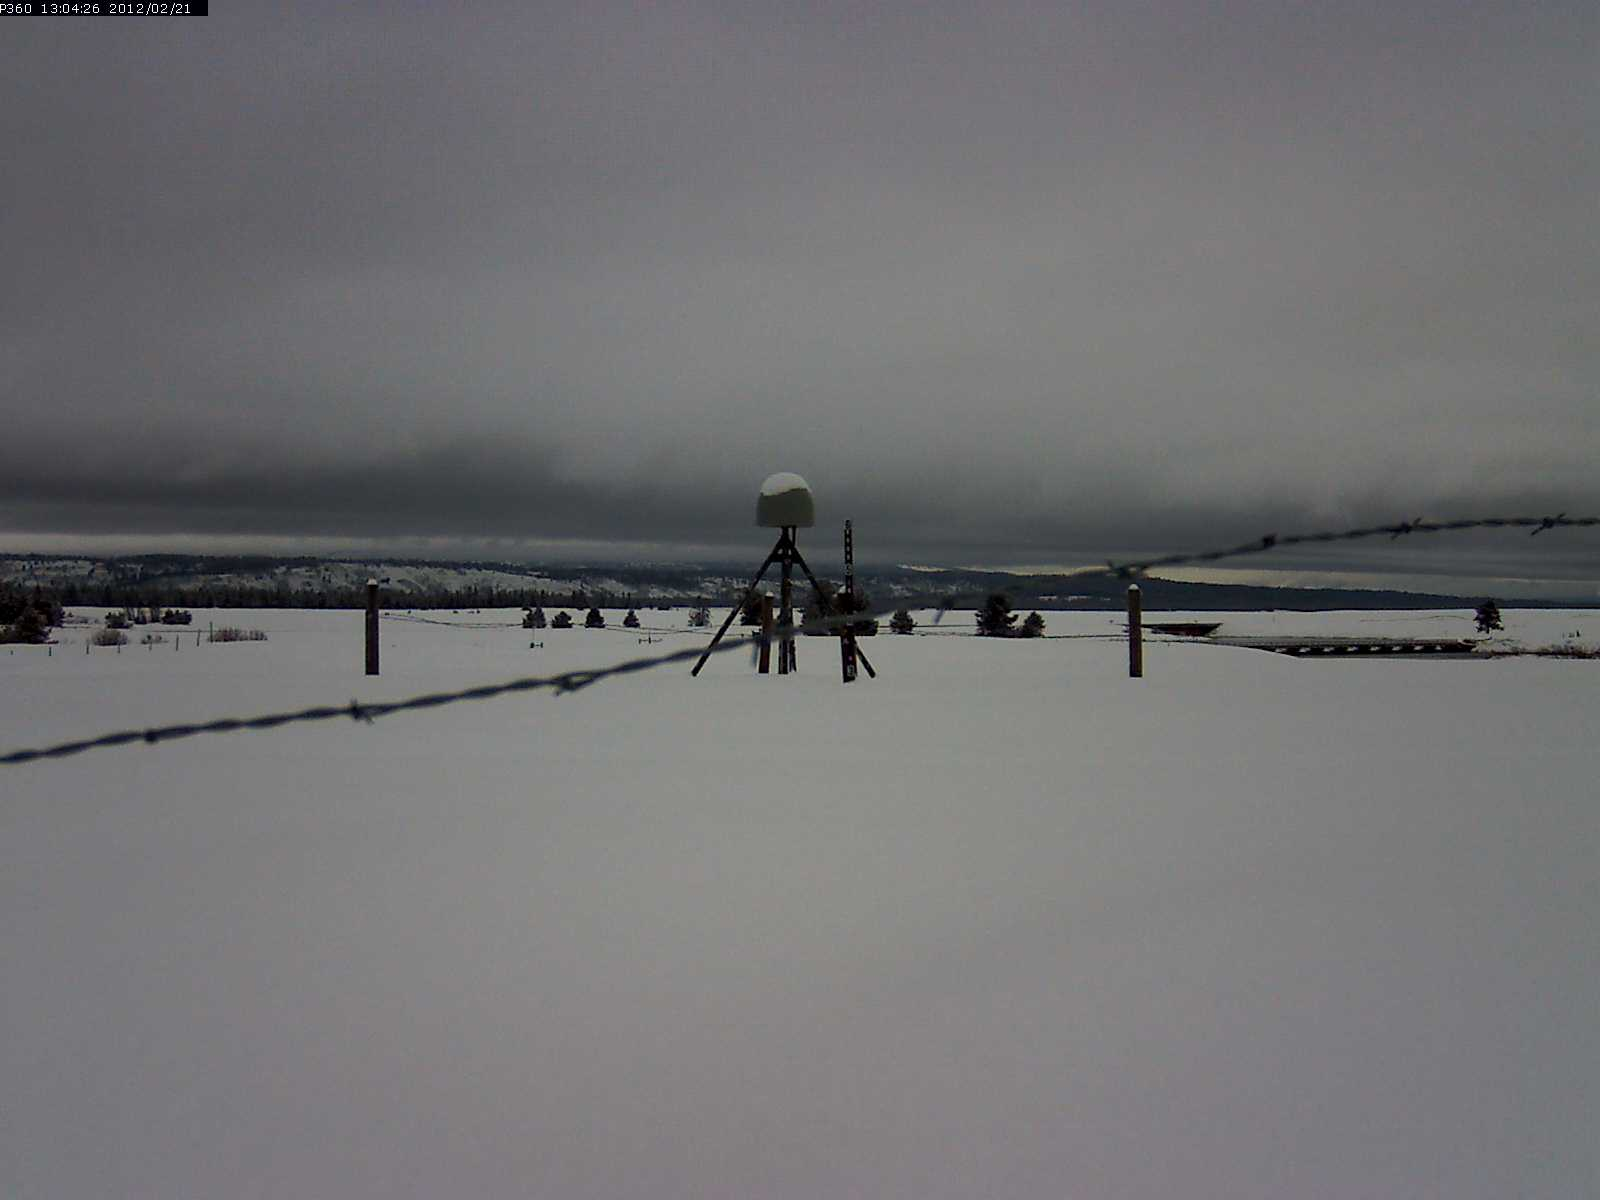
\includegraphics[width=9\linewidth,trim=100 600 100 600]{img/P36020120221_130426M.jpg}
\end{frame}

%---  p360 site photo frame -------------------------%
\begin{frame}{P360 - Feb 22}
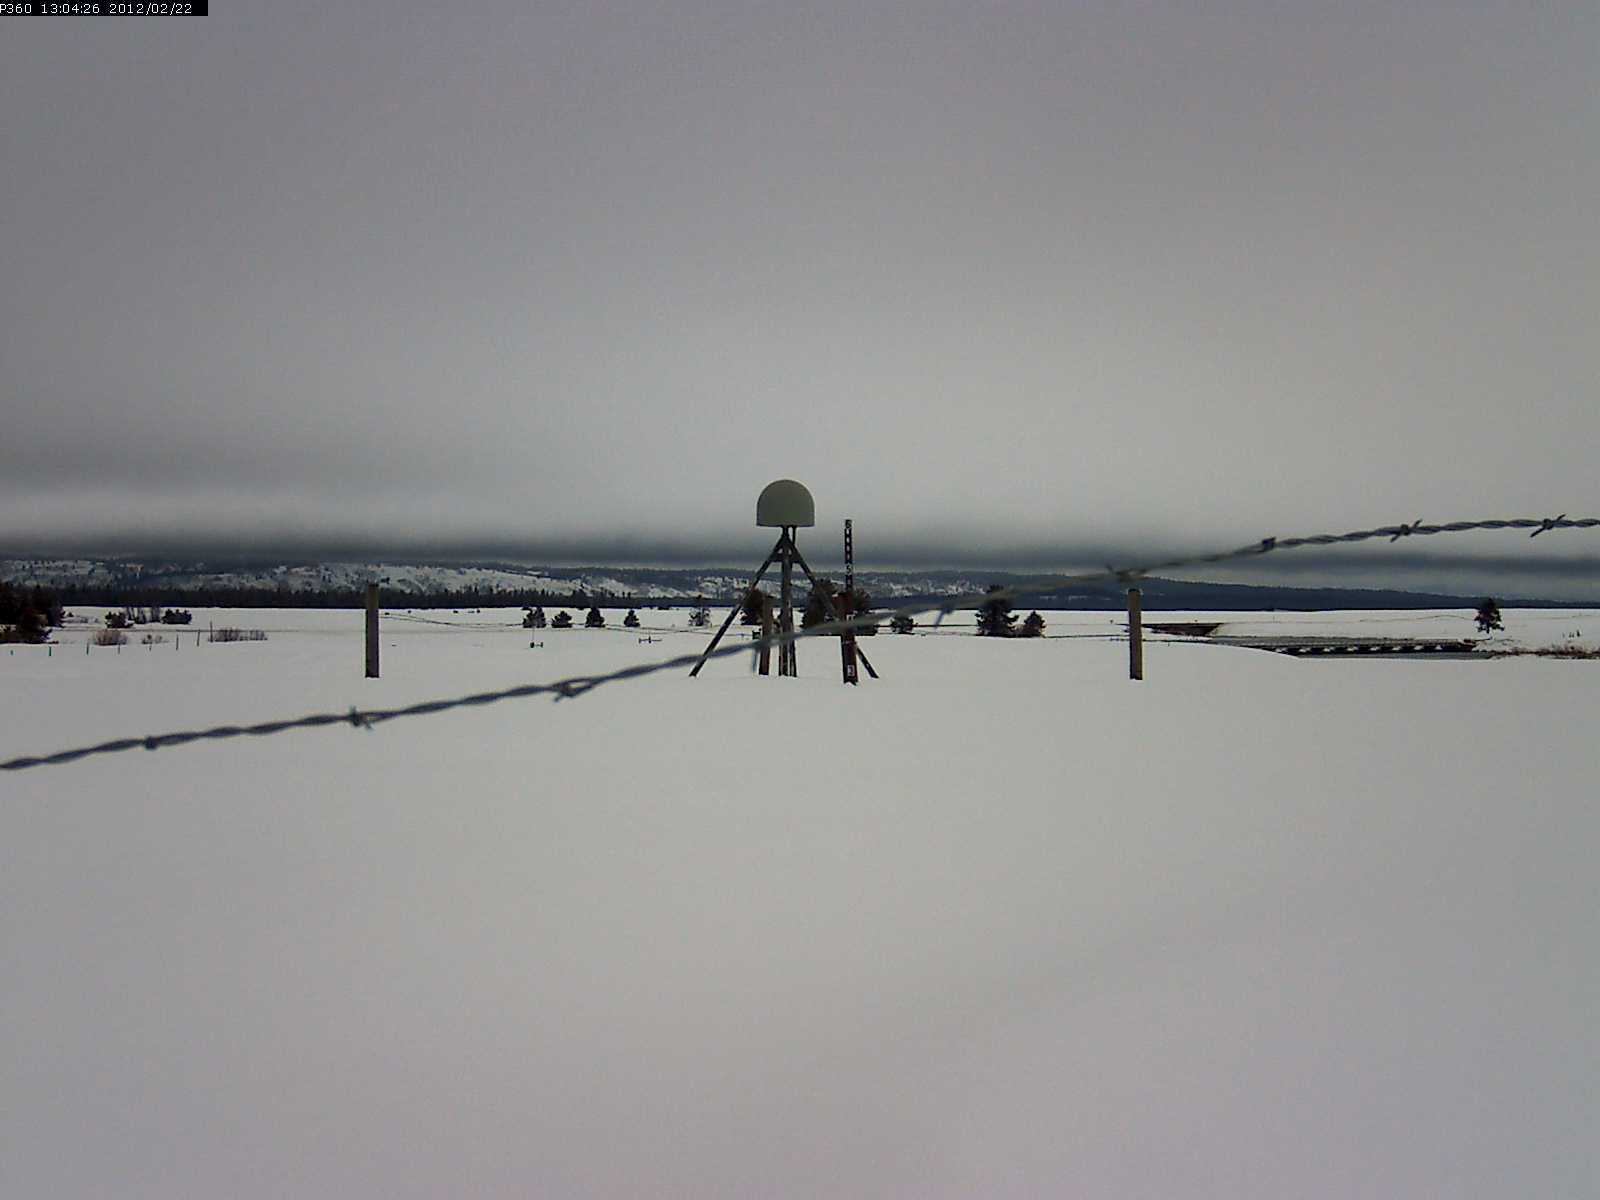
\includegraphics[width=9\linewidth,trim=100 600 100 600]{img/P36020120222_130426M.jpg}
\end{frame}


%---data considered  frame -------------------------%
\begin{frame}{Data Used}
\begin{itemize}
  \item Data with snow on antenna: Feb 21
  \item Data without any snow on antena: Feb 22
  \item Satellite Track Used: PRN17 
    \begin{itemize}
      \item visible around the same time the photos were taken
      \item rises upto $89.4^o$
      \item has L2c
    \end{itemize}
\end{itemize}
\end{frame}


%---parameters  frame -------------------------%
\begin{frame}{Parameters}
\begin{itemize}
  \item $MP_1$
  \item Signal to Noise Ratio (SNR)
  \item Position Time Series
\end{itemize}
\end{frame}

%---SNR  frame -------------------------%
\begin{frame}{SNR}
Heuristic
\begin{itemize}
  \item Accumulate SNR data as a function of elevation and PRN to generate an expectation map.
  \item Use above data as a control data set to indicate if received signal power is lower than expected.
  \item Can indicate snow cover.
\end{itemize}
\end{frame}
\begin{frame}{SNR}
Model
\begin{itemize}
  \item Use simple EM model to calculate signal loss through a slab of snow.
  \item estimate the snow cover over antenna by comparing with the signal loss from direct signal power.
\end{itemize}
\end{frame}
\end{frame}

% \begin{frame}{SNR}
% Modeled II
% \begin{itemize}
%   \item Extract Phase and Amplitude from lomb-scargle retrievals.
%   \item Expected SNR [\ref{todo}] \begin{equation}SNR=A\sin(\frac{2\pi h}{\lambda}sin(el) + \phi)\end{equation} 
%   \item Can power loss be estimated from the above two?
%   \item Amplitude of modeled SNR does not vary with elevation.
% \end{itemize}
% \end{frame}

%---snr plots  frame -------------------------%
\begin{frame}{SNR Plots}
  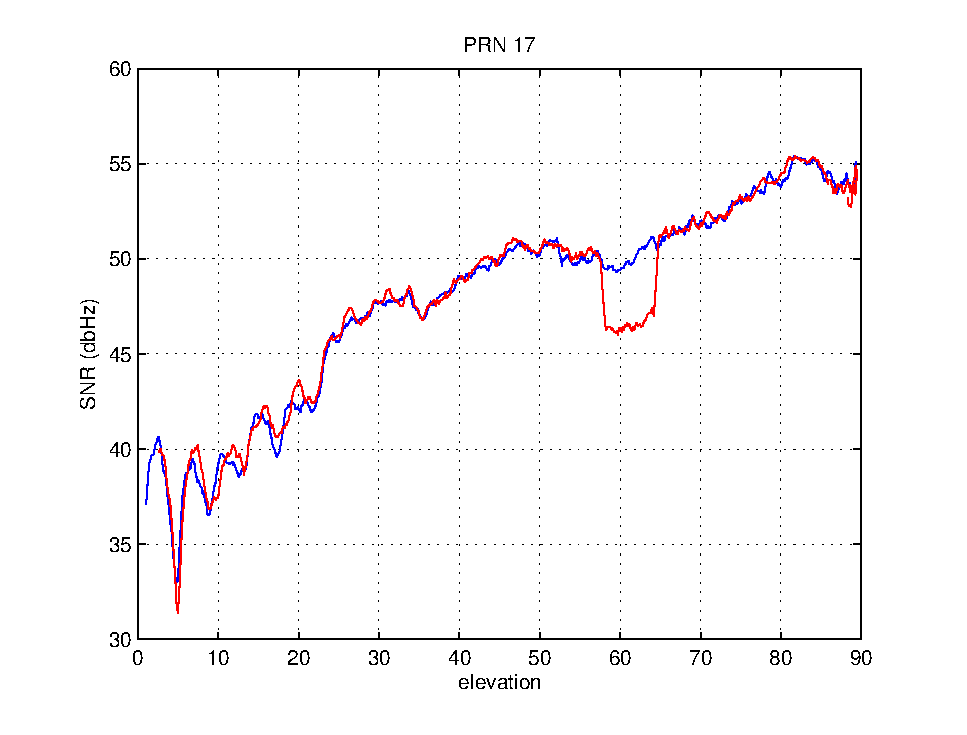
\includegraphics[width=1\linewidth]{img/snr_prn17_smth.eps}
\end{frame}
\begin{frame}{SNR Plots}
  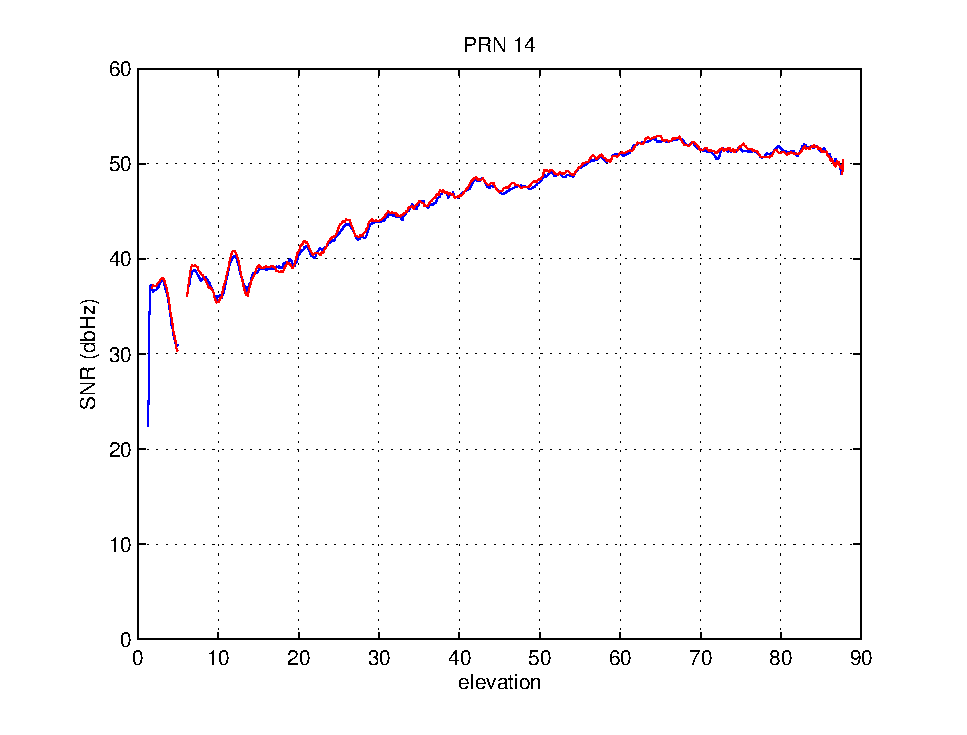
\includegraphics[width=1\linewidth]{img/snr_prn14_smth.eps}
\end{frame}
\begin{frame}{SNR Plots}
  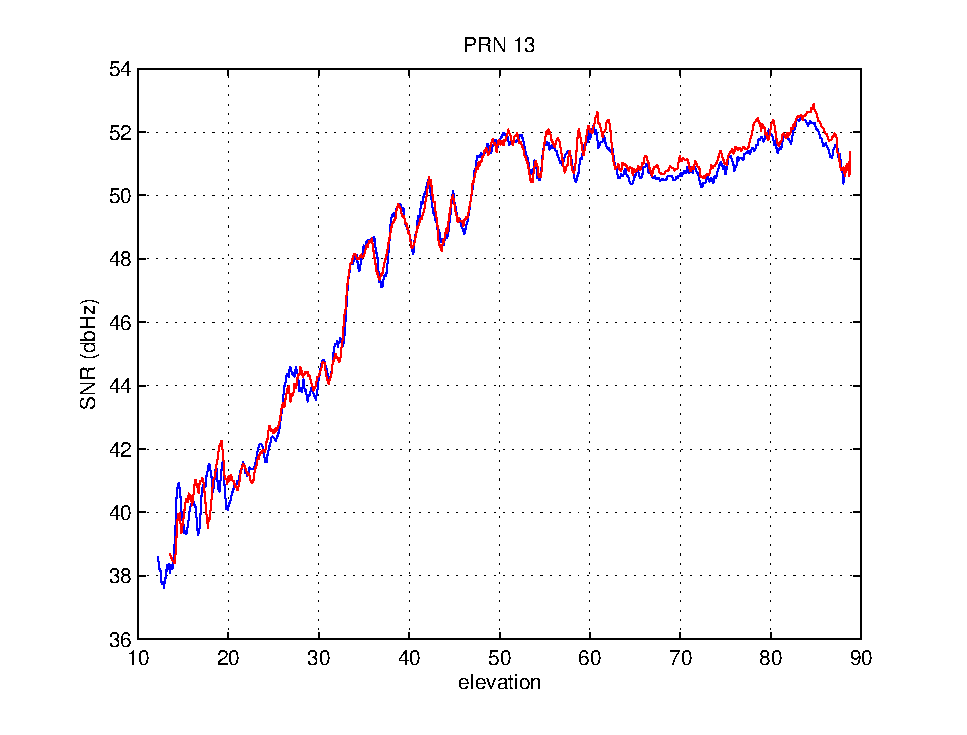
\includegraphics[width=1\linewidth]{img/snr_prn13.eps}
\end{frame}


%---  frame -------------------------%
\begin{frame}{}
\end{frame}

\end{document}